% ---------- Titelblad Masterproef Faculteit Wetenschappen -----------
% Dit document is opgesteld voor compilatie met pdflatex.  Indien je
% wilt compileren met latex naar dvi/ps, dien je de figuren naar
% (e)ps-formaat om te zetten.
%                           -- december 2012
% -------------------------------------------------------------------
\RequirePackage{fix-cm}
\documentclass[12pt,a4paper,oneside]{article}

% --------------------- In te laden pakketten -----------------------
% Deze kan je eventueel toevoegen aan de pakketten die je al inlaadt
% als je dit titelblad integreert met de rest van thesis.
% -------------------------------------------------------------------
\usepackage{graphicx,xcolor,textpos}
\usepackage{helvet}

% -------------------- Pagina-instellingen --------------------------
% Indien je deze wijzigt, zal het titelblad ook wijzigen.  Dit dien je
% dan manueel aan te passen.
% --------------------------------------------------------------------

\topmargin -10mm
\textwidth 160truemm
\textheight 240truemm
\oddsidemargin 0mm
\evensidemargin 0mm

% ------------------- textpos-instellingen ---------------------------
% Enkele andere instellingen voor het voorblad.
% --------------------------------------------------------------------

\definecolor{green}{RGB}{172,196,0}
\definecolor{bluetitle}{RGB}{29,141,176}
\definecolor{blueaff}{RGB}{0,0,128}
\definecolor{blueline}{RGB}{82,189,236}
\setlength{\TPHorizModule}{1mm}
\setlength{\TPVertModule}{1mm}



%----------------------- Custom stuff -------------------------------

\graphicspath{./}
\usepackage{makeidx}
\index{hoofd}
\makeindex
\usepackage{amsmath}
\usepackage[dutch]{babel}

\usepackage{hyperref}
\usepackage{graphicx}
\usepackage{caption}
\usepackage{subcaption}




%------------------------ Plot packages ----------------------------
\usepackage{tikz}
\usepackage{pgfplots}

\usepackage{pgf}
\usepackage{units}
\usepackage{metalogo}







% --------------------------------------------------------------------


\title{Project wavelets}
\author{Matthias Baeten \& Bob Vergauwen}
\date{ 13 januari 2016}

\begin{document}

\maketitle

\section{Ruisreductie}


\section{Inpainting}

\begin{figure}
    \centering
    \begin{subfigure}[b]{0.45\textwidth}
        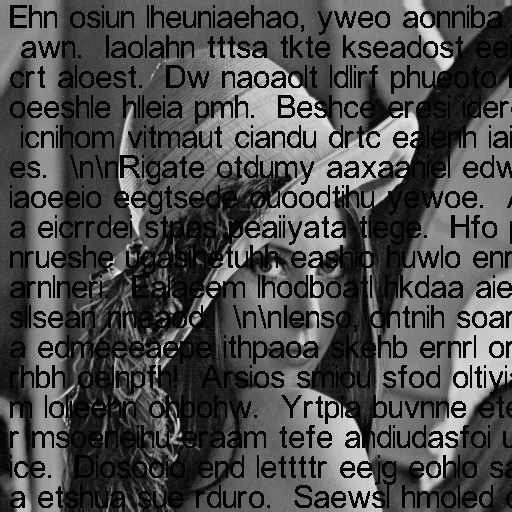
\includegraphics[width=\textwidth]{../src/inpainting/lena_broke}
        \caption{Met tekst beschadiging}
        \label{fig:tiger}
    \end{subfigure}
    ~ %add desired spacing between images, e. g. ~, \quad, \qquad, \hfill etc. 
    %(or a blank line to force the subfigure onto a new line)
    \begin{subfigure}[b]{0.45\textwidth}
        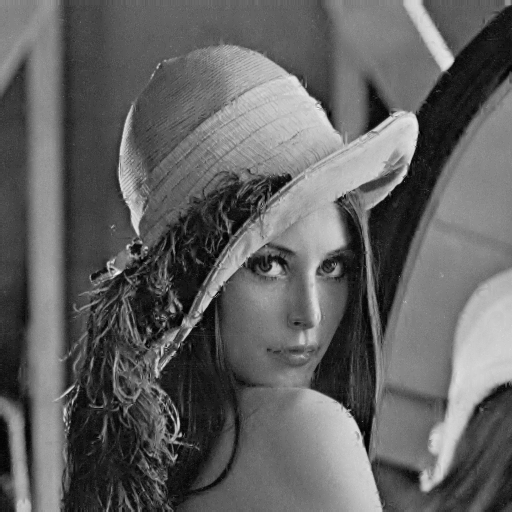
\includegraphics[width=\textwidth]{../src/inpainting/lena_fixed}
        \caption{Na de reconstructie}
        \label{fig:mouse}
    \end{subfigure}
    \caption{Pictures of lena}\label{fig:animals}
\end{figure}




\begin{figure}
    \centering
    \begin{subfigure}[b]{0.45\textwidth}
        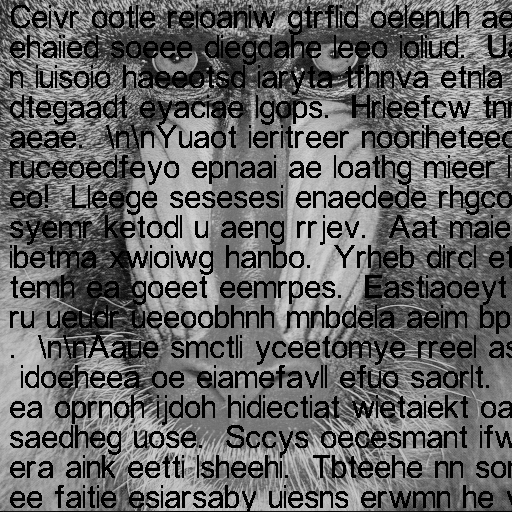
\includegraphics[width=\textwidth]{../src/inpainting/baboon_broke}
        \caption{Met tekst beschadiging}
        \label{fig:tiger}
    \end{subfigure}
    ~ %add desired spacing between images, e. g. ~, \quad, \qquad, \hfill etc. 
    %(or a blank line to force the subfigure onto a new line)
    \begin{subfigure}[b]{0.45\textwidth}
        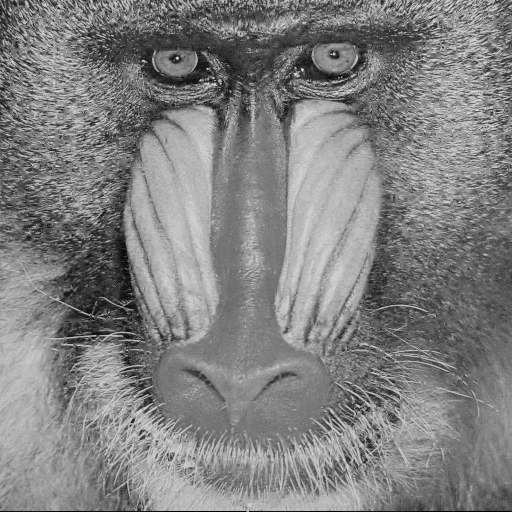
\includegraphics[width=\textwidth]{../src/inpainting/baboon_fixed}
        \caption{Na de reconstructie}
        \label{fig:mouse}
    \end{subfigure}
    \caption{Pictures of lena}\label{fig:baboon}
\end{figure}


\begin{figure}
    \centering
    \begin{subfigure}[b]{0.45\textwidth}
        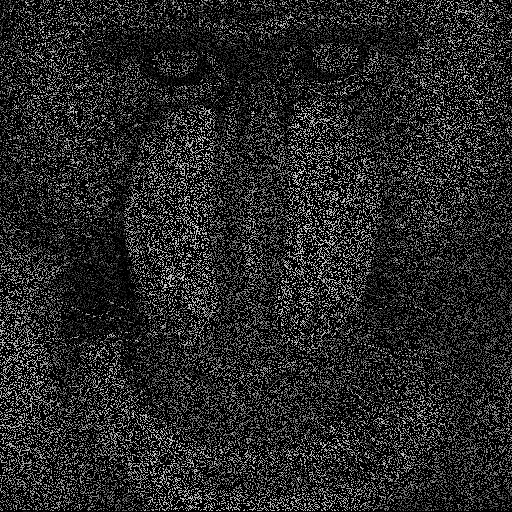
\includegraphics[width=\textwidth]{../src/inpainting/baboon_broke_random}
        \caption{Met random beschadiging (70 procent)}
        \label{fig:tiger}
    \end{subfigure}
    ~ %add desired spacing between images, e. g. ~, \quad, \qquad, \hfill etc. 
    %(or a blank line to force the subfigure onto a new line)
    \begin{subfigure}[b]{0.45\textwidth}
        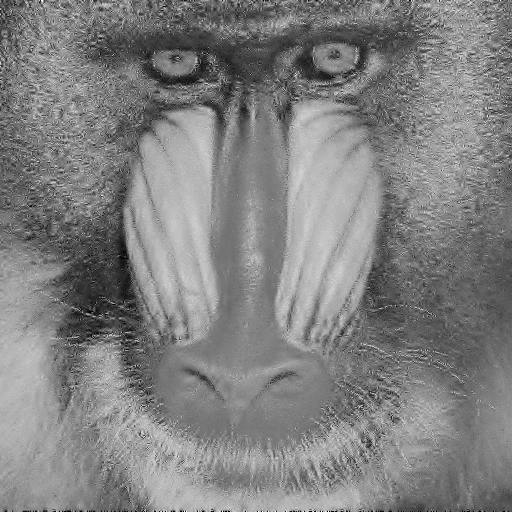
\includegraphics[width=\textwidth]{../src/inpainting/baboon_fixed_random}
        \caption{Na de reconstructie}
        \label{fig:mouse}
    \end{subfigure}
    \caption{Pictures of lena}\label{fig:baboon}
\end{figure}


\begin{figure}
    \centering
    \begin{subfigure}[b]{0.45\textwidth}
        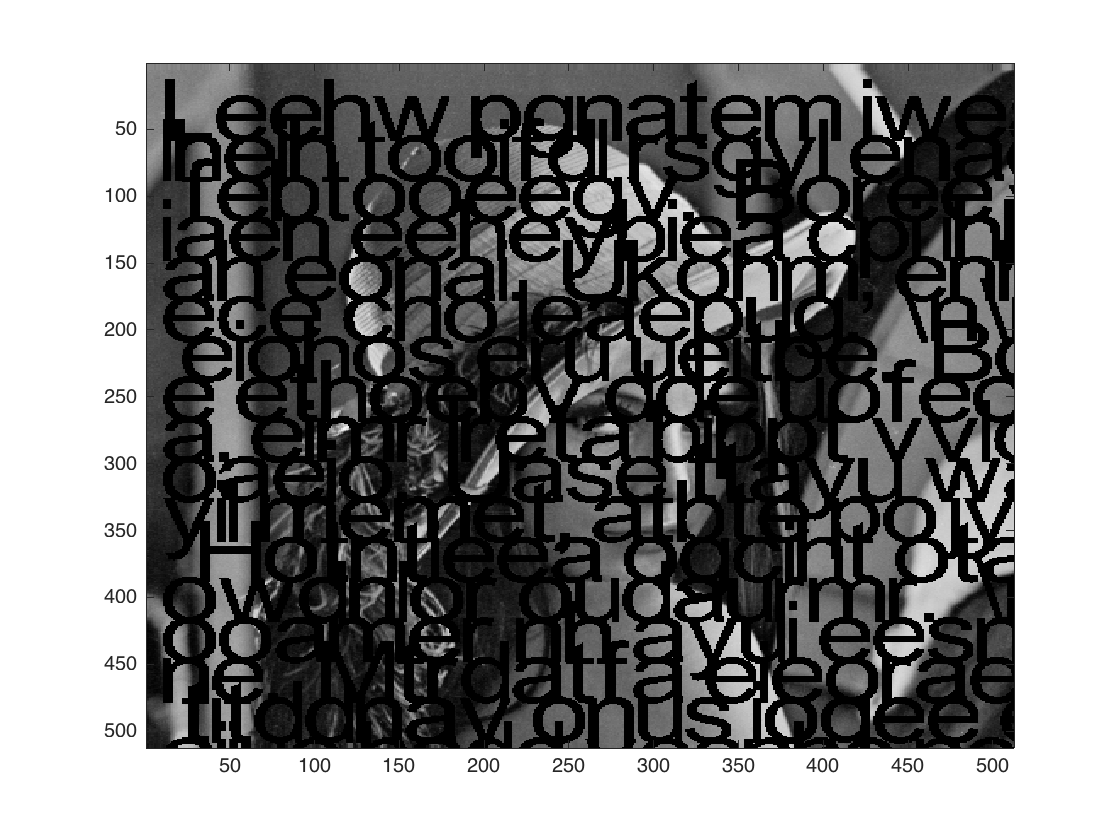
\includegraphics[width=\textwidth]{../src/inpainting/lena_broke2}
        \caption{tekstbeschadigde figuur. \\ \ \\ \ \\ \ \\ \ \\}
        \label{fig:fig1}
    \end{subfigure}
    ~ %add desired spacing between images, e. g. ~, \quad, \qquad, \hfill etc. 
    %(or a blank line to force the subfigure onto a new line)
    \begin{subfigure}[b]{0.45\textwidth}
        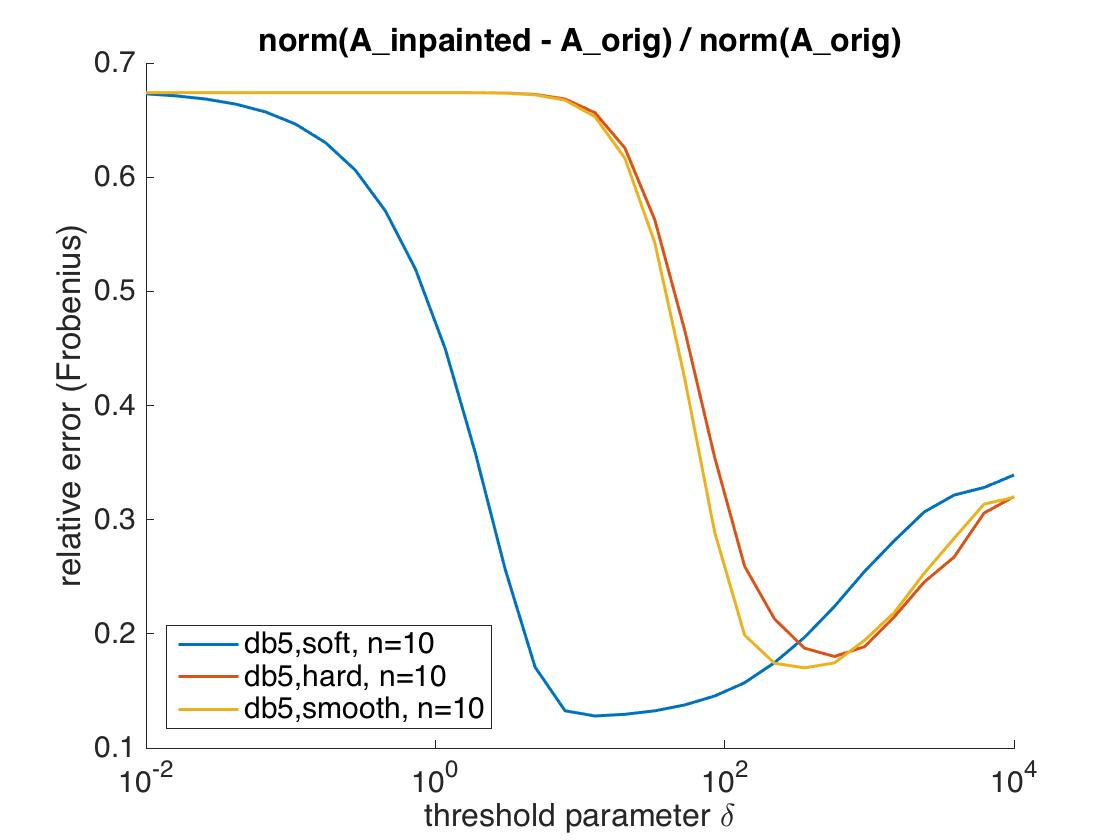
\includegraphics[width=\textwidth]{../src/inpainting/paint_letters_db5_threskinds_it50}
        \caption{Voor verschillende waarden van de threshold parameter $\delta$ is de figuur ingepaint met telkens $50$ iteraties. De relatieve fout t.o.v. de onbeschadigde figuur is telkens berekent.}
        \label{fig:mouse}
    \end{subfigure}
      \begin{subfigure}[b]{0.45\textwidth}
        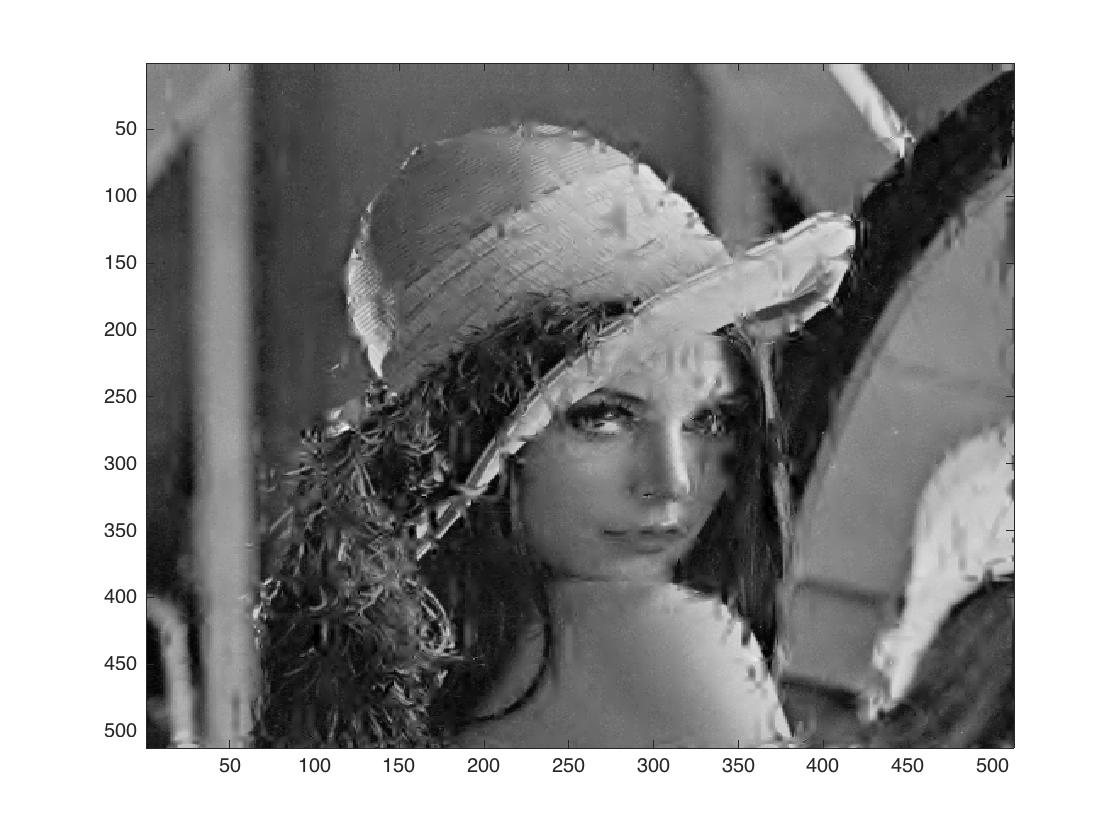
\includegraphics[width=\textwidth]{../src/inpainting/soft_succeed}
        \caption{figuur \ref{fig:fig1} ingepaint met 'db5' wavelets. Soft thresholding is gebruikt met parameter $\delta = 10$. Hier is het goed gelukt, de blauwe curve bereikt zijn mimimum rond $\delta = 10$. \\}
        \label{fig:tiger}
    \end{subfigure}
    ~ %add desired spacing between images, e. g. ~, \quad, \qquad, \hfill etc. 
    %(or a blank line to force the subfigure onto a new line)
    \begin{subfigure}[b]{0.45\textwidth}
        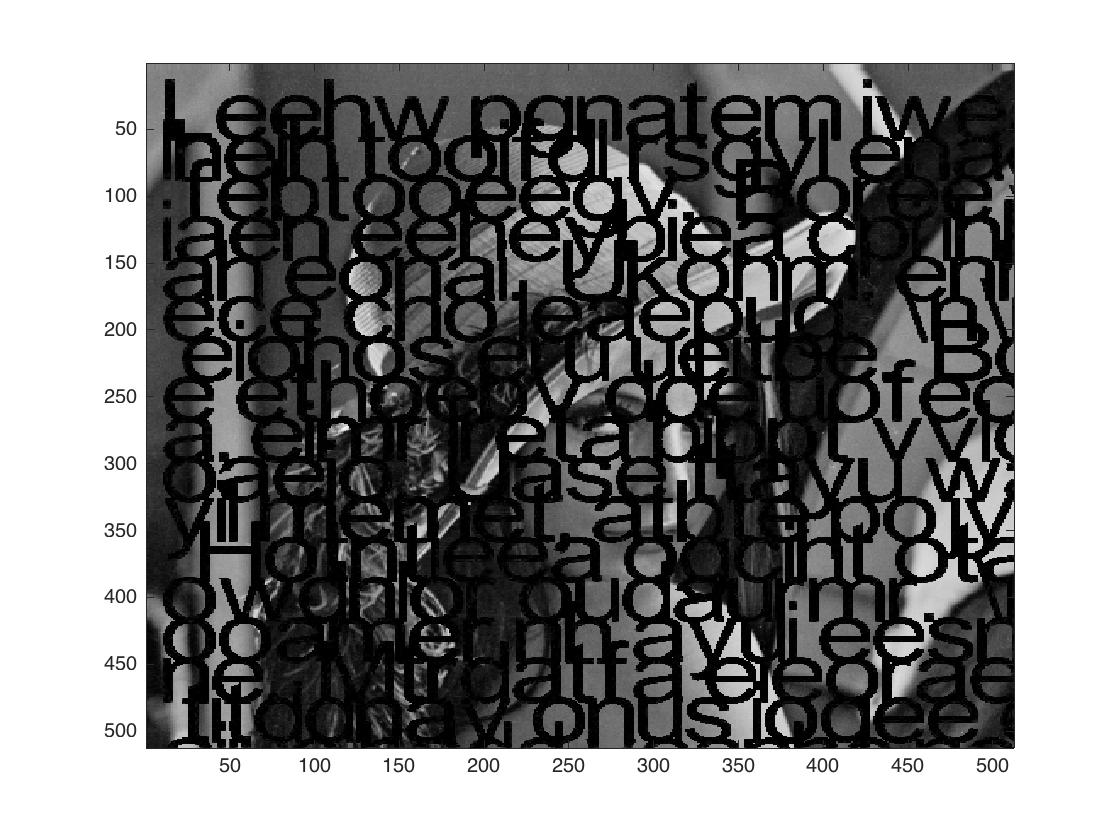
\includegraphics[width=\textwidth]{../src/inpainting/hard_fail}
        \caption{figuur \ref{fig:fig1} ingepaint met 'db5' wavelets. Hard thresholding is gebruikt met parameter $\delta = 10$. Hier is het mislukt. De reden hiervoor is dat de  rode curve voor $\delta = 10$ totaal niet het mimimum bereikt.}
        \label{fig:mouse}
    \end{subfigure}
    \caption{Effect van threshold parameter en threshold techniek bij inpainting}\label{fig:baboon}
\end{figure}

\begin{figure}
    \centering
    \begin{subfigure}[b]{0.7\textwidth}
        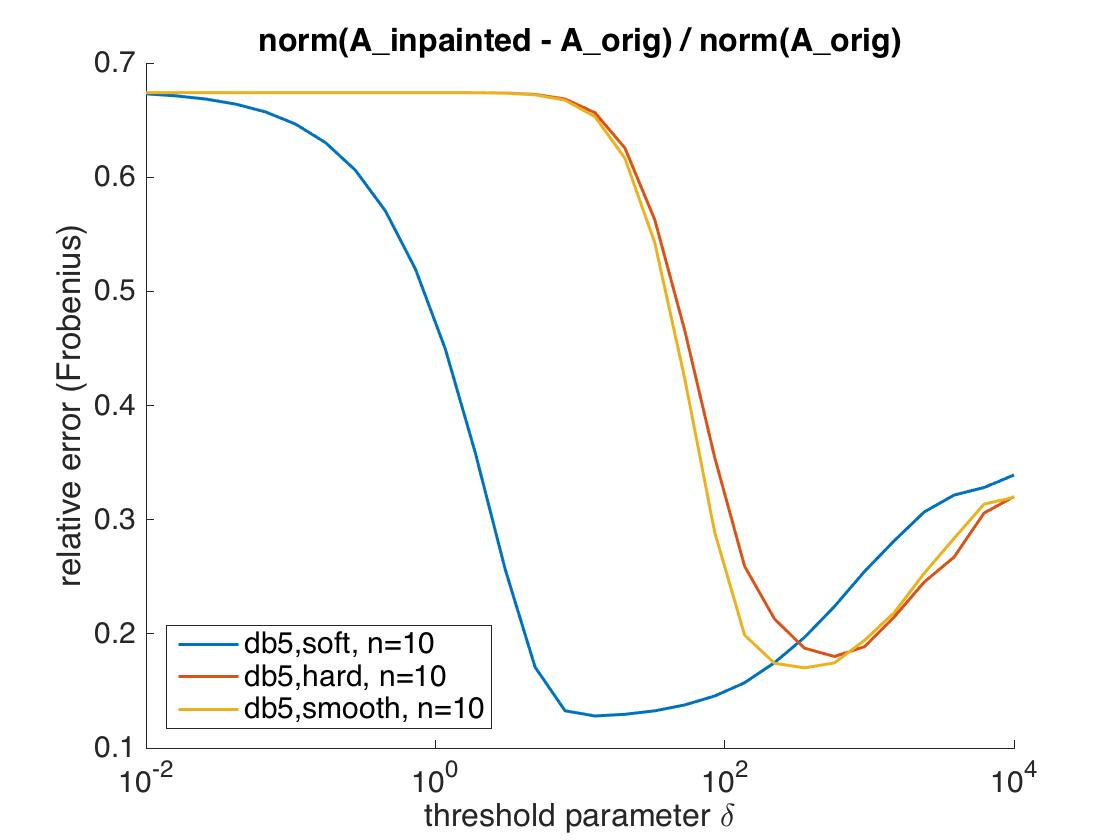
\includegraphics[width=\textwidth]{../src/inpainting/paint_letters_db5_threskinds_it50}
        \caption{Voor verschillende waarden van de threshold parameter $\delta$ is de figuur ingepaint met telkens $50$ iteraties. De relatieve fout t.o.v. de onbeschadigde figuur is telkens berekent. verschillende threshold technieken zijn gebruikt.(dezelfde figuur als vorige pagina)}
        \label{fig:tiger}
    \end{subfigure}
    ~ %add desired spacing between images, e. g. ~, \quad, \qquad, \hfill etc. 
    %(or a blank line to force the subfigure onto a new line)
    \begin{subfigure}[b]{0.7\textwidth}
        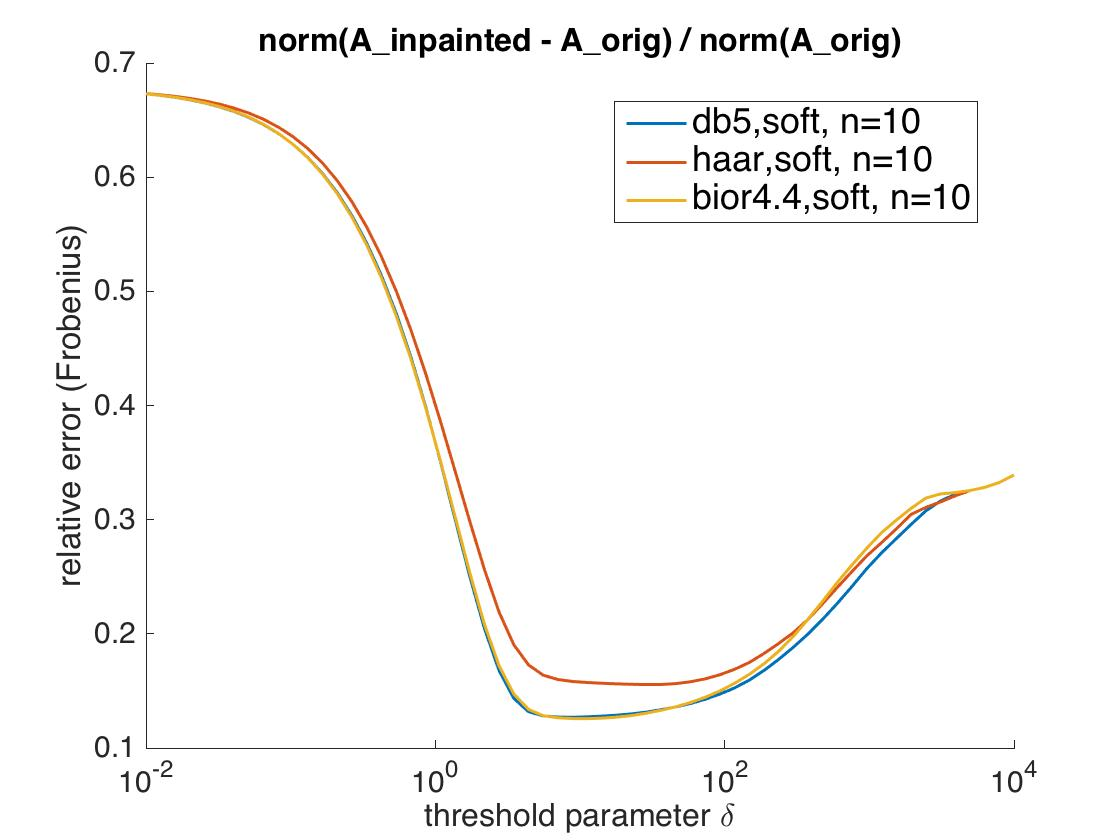
\includegraphics[width=\textwidth]{../src/inpainting/paint_letter_wavekinds_soft_it50}
        \caption{Voor verschillende waarden van de threshold parameter $\delta$ is de figuur ingepaint met telkens $50$ iteraties. De relatieve fout t.o.v. de onbeschadigde figuur is telkens berekent.verschillende soorten wavelets zijn gebruikt.}
        \label{fig:mouse}
    \end{subfigure}
    \caption{plots error vs $\delta$}\label{fig:baboon}
\end{figure}


\begin{figure}
    \centering
    \begin{subfigure}[b]{0.7\textwidth}
        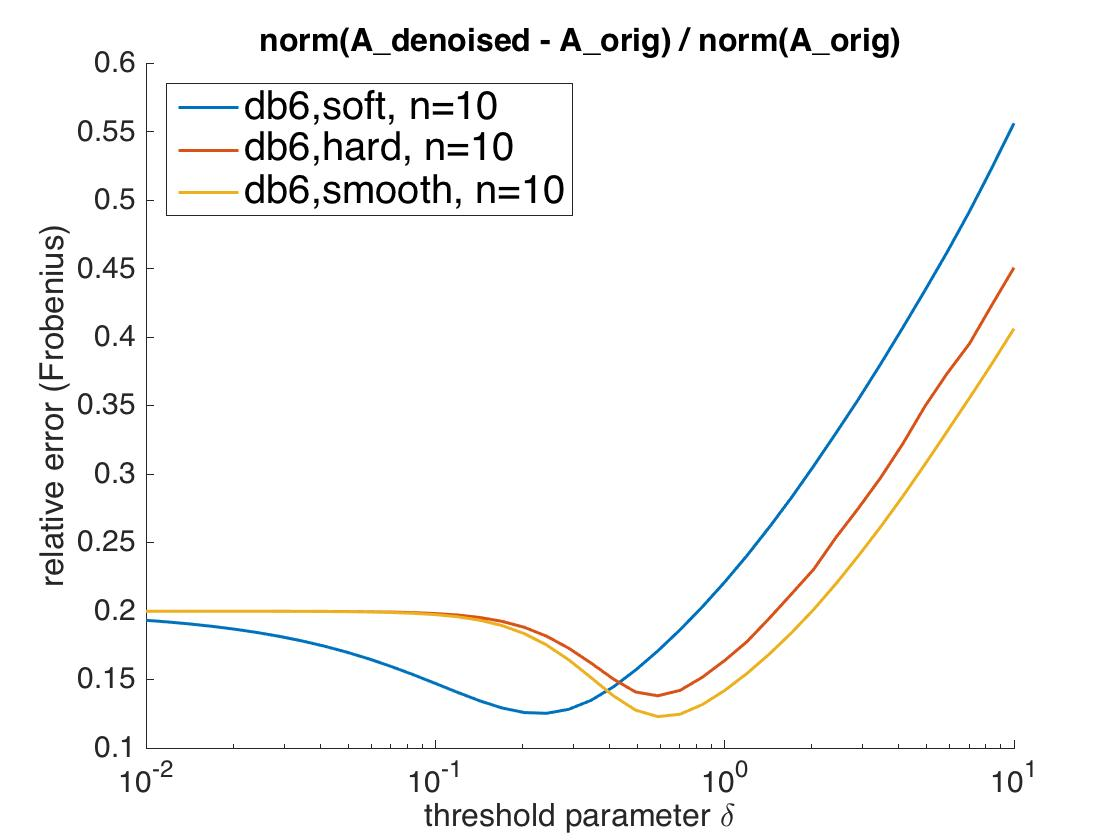
\includegraphics[width=\textwidth]{../src/denoising/denoised_err_threskinds}
        \caption{Voor verschillende waarden van de threshold parameter $\delta$ is een noisy figuur gedenoised. De relatieve fout t.o.v. de originele figuur(zonder noise) is telkens berekent. verschillende threshold technieken zijn gebruikt. De onbewerkte noisy figuur heeft een relatieve fout van $0.2$. Conclusie: opletten met de waarde van de threshold parameter.}
        \label{fig:tiger}
    \end{subfigure}
    ~ %add desired spacing between images, e. g. ~, \quad, \qquad, \hfill etc. 
    %(or a blank line to force the subfigure onto a new line)
    \begin{subfigure}[b]{0.7\textwidth}
        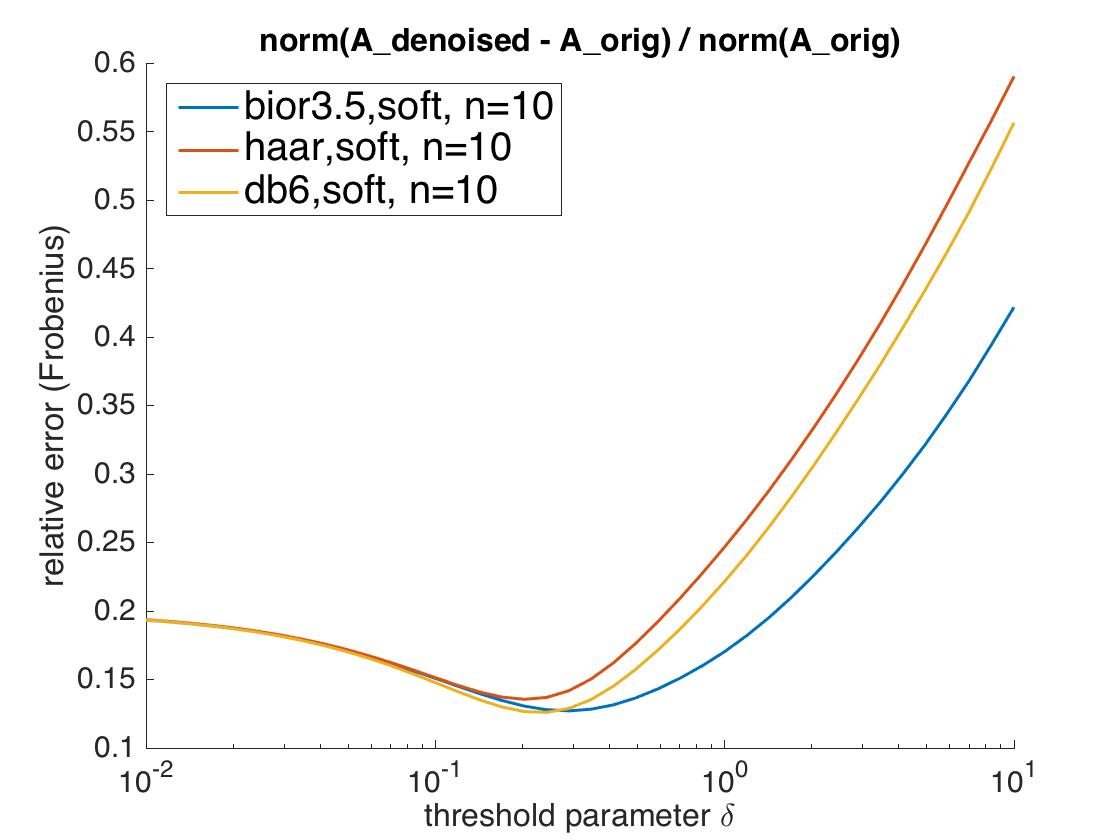
\includegraphics[width=\textwidth]{../src/denoising/denoised_err_wavekinds}
        \caption{Voor verschillende waarden van de threshold parameter $\delta$ is een noisy figuur gedenoised. De relatieve fout t.o.v. de originele figuur(zonder noise) is telkens berekent. De onbewerkte noisy figuur heeft een relatieve fout van $0.2$.verschillende soorten wavelets zijn gebruikt. Conclusie: opletten met de waarde van de threshold parameter..}
        \label{fig:mouse}
    \end{subfigure}
    \caption{plots error vs $\delta$}\label{fig:baboon}
\end{figure}

\end{document}
